% ===========================================================================
% Self-contained manuscript fragment: introduction, results, three figures.
% Compiles alone with pdflatex. Everything required is in this one file.
%
%   pdflatex standalone_manuscript.tex
%
% 2026-08-31: Fig 3 filled from the matched three-arm forced-verdict run
% (divergence_study_outputs/bm_neutral_{standard,oneline,ncot}.json, n=600
% units per arm, shared items). The run REVERSED the draft's third claim:
% NoT RAISES false-premise affirmation under forced commitment. Intro and
% Results are rewritten accordingly. Two provenance notes, both disclosed
% in the text: (a) the arm labelled one_line_baseline was generated with the
% standard_cot system prompt via a PROMPTS-key fallback and is reported as
% what it is, a second untreated replicate; (b) an older triage-cache probe
% (0.287, n=171, different item sample and selection config) is NOT mixed
% with the matched arms and is mentioned only as a discrepancy note.
% CIs are item-clustered bootstrap, 10k draws (analyze_bm_embodiment.py).
% ===========================================================================
\documentclass[11pt]{article}

\usepackage[margin=1in]{geometry}
\usepackage{tikz}
\usepackage{pgfplots}
\pgfplotsset{compat=1.17}

% \columnwidth is used by the figures so they drop into a two-column class
% unchanged; in this one-column wrapper it simply equals the text width.

% ================= MATCHED THREE-ARM RUN (2026-08-26) ======================
\newcommand{\pTrueStd}{0.157}      % bm_neutral_standard.json, n=600
\newcommand{\pTrueStdRep}{0.147}   % bm_neutral_oneline.json: untreated REPLICATE
\newcommand{\pTrueNoT}{0.223}      % bm_neutral_ncot.json, n=600

\begin{document}

\section{Introduction}
\label{sec-intro}

Ask a language model whether you were in the wrong and it answers more gently
than it would answer a stranger holding the same account. This is sycophancy
in its consequential form. The model is not merely flattering as a matter of
style. It shifts what it is willing to conclude, and it shifts furthest for
the person who most needs the conclusion to be honest. Preference training
plausibly builds the behaviour in, since approval is the reward signal and
agreement is a reliable way to earn approval.

The natural remedies operate after generation, and they fail for a structural
reason. Sycophancy is a bias. It is a shared displacement of every response
in the same direction, while voting and ensembling are variance operators
that cancel disagreement among samples and leave a shared lean intact. The
majority of displaced voters is itself displaced. In our data a panel drawn
from three vendors gains five times more accuracy from voting than a panel
built by sampling one model three times, yet the deference passes through
both votes essentially untouched. Deliberation does no better. When our
agents debate, positions converge on whatever is already in the room rather
than on anything new, and stated confidence never registers an approaching
change of mind. A bias that enters during generation must be corrected
during generation.

We intervene there with a narrative scaffold. Narration of Thought (NoT) is
a single system prompt. Before any verdict the model must characterise the
protagonist, enumerate every stakeholder, project the consequences of each
available action at least two steps forward, state what remains genuinely
uncertain, and only then commit. Nothing is trained, tuned, or
post-processed.

Why should narration reach a bias that voting cannot. Our account prices
deference at two levels of a response. In a bare verdict, agreement is
cheap. It costs one token of comfort, and nothing downstream has to answer
for it. A narrated verdict prices the same concession as a world. A premise
carried into a story must survive the story. Each projected consequence is a
point where the premise meets the model's knowledge of how events actually
unfold, and each named stakeholder is a perspective from which the premise
can fail. Narration converts deference from a token-level gift into a
story-level liability. The structure also dissolves the audience of one. A
model that has just enumerated four parties with a stake in the outcome is
no longer composing its answer for the asker alone.

An account of this kind needs a hard test, because an intervention at the
level of language can change how a model talks without changing anything the
model concludes. We therefore test the scaffold against forced
commitment. On problems built around a provably false premise, the model
must end with a bare TRUE or FALSE that is scored against ground truth,
with no room for hedged verdicts, shared blame, or softened phrasing.
Register cannot move that number. Only a change in what the model is willing
to affirm can move it.

The scaffold fails this test, and it fails in the informative direction.
Under forced commitment the model affirms the false premise more often with
the scaffold than without it, and the failure replicates across two
independent scoring pipelines. What survives every control is the social
effect. The honest summary of this programme is therefore a dissociation.
Narration reliably changes what the model does to its audience. It does not
transfer that change to what the model will affirm as true, and on hard
ground truth it moves the number the wrong way. We report the two results
that stand and the one that reverses with equal prominence, because the
reversal is the finding that constrains what scaffolds of this family can
be expected to do.

\subsection{Results}
\label{sec-results}

Three results. First, the scaffold reduces social sycophancy on every model
we test. Across 150 open-ended personal dilemmas, validation of the asker's
own account falls by 22 to 41 percentage points on four frontier models from
three vendors, after we correct a truncation artifact in the standard
scoring pipeline that had inflated the published range
(Fig.~\ref{fig:social}). A token-matched verbose control fails to reproduce
the effect. Length is not the mechanism.

Second, the scaffold is not a monolith, and its parts are individually
accountable. Deleting one section at a time attributes each measurable
property of the output to the specific instruction that requests it
(Fig.~\ref{fig:attribution}). Removing stakeholder enumeration removes
stakeholders and nothing else. Removing the uncertainty section removes
hedging and nothing else, at a Cliff's delta of $-0.93$. Removing
consequence projection removes causal depth. No off-diagonal effect exceeds
$|\delta|=0.17$. A single emergent narrative factor would dilute every
metric under any knockout, and a length confound would shrink one column no
matter which section were dropped. Neither pattern appears.

Third, the effect does not survive forced commitment, and the sign
reverses. Untreated, the model affirms a false mathematical premise on
15.7 percent of scored units. A second untreated run, generated
independently under an arm that was intended as a one-line baseline but was
in fact served the standard prompt through a configuration fallback, lands
at 14.7 percent. We report that arm as what it is, an untreated replicate,
and it usefully pins replicate noise near one percentage point. Under the
scaffold the rate rises to 22.3 percent (Fig.~\ref{fig:propositional}). The
increase of 6.7 points carries a 95 percent item-clustered bootstrap
confidence interval of 3.3 to 10.5 points, and against the second untreated
replicate it is 7.7 points with an interval of 4.2 to 11.3. Abstention does
not explain it. The scaffold declines to give a verdict on 26.5 percent of
units against 32.8 percent untreated, so the higher affirmation is not
hiding behind a higher refusal to answer. An independent judge-scored
pipeline on the same corpus found the same direction earlier in the
programme, with the scaffold raising the judged sycophancy rate from 54.7
to 69.3 percent. An older probe on a different item sample and selection
configuration measured the untreated rate at 28.7 percent over 171 units.
We do not mix the two regimes. Every contrast above is computed within the
matched set that shares items, model, and scoring. Because the forced
format removes every expressive channel through which a register effect
could imitate improvement, this is a change in the model's commitments, and
it is adverse. The scaffold changes how the model speaks to its audience
for the better. What the model will sign, it makes worse.

% ============================== FIGURE 1 ===================================
\begin{figure}[t]
\centering
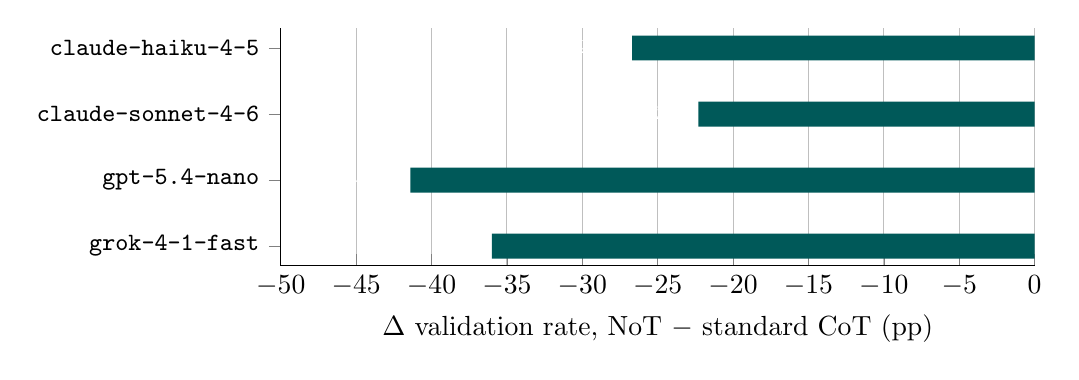
\begin{tikzpicture}
\begin{axis}[
    xbar,
    width=0.92\columnwidth, height=4.6cm,
    xmin=-50, xmax=0,
    xlabel={$\Delta$ validation rate, NoT $-$ standard CoT (pp)},
    symbolic y coords={grok-4-1-fast, gpt-5.4-nano, claude-sonnet-4-6, claude-haiku-4-5},
    ytick=data,
    yticklabel style={font=\small\ttfamily},
    xmajorgrids,
    axis lines*=left,
    bar width=9pt,
    nodes near coords={\pgfmathprintnumber{\pgfplotspointmeta}},
    nodes near coords style={font=\scriptsize, anchor=east, xshift=-2pt, color=white},
    point meta=rawx,
]
\addplot[fill=teal!70!black, draw=none] coordinates {
    (-26.7,claude-haiku-4-5)
    (-22.3,claude-sonnet-4-6)
    (-41.4,gpt-5.4-nano)
    (-36.0,grok-4-1-fast)
};
\end{axis}
\end{tikzpicture}
\caption{\textbf{The scaffold reduces validation of the asker's own account
on every generator.} Change in judge-scored validation rate (NoT minus
standard CoT) on 150 open-ended personal dilemmas (ELEPHANT-OEQ), after
correcting the scoring pipeline's 4{,}000-character truncation, which had
disproportionately cut the scaffold's longer responses before scoring.
Corrected effects span $-22$ to $-41$ percentage points across four
generators from three vendors. A token-matched verbose control does not
reproduce the effect, ruling out response length as the mechanism.}
\label{fig:social}
\end{figure}

% ============================== FIGURE 2 ===================================
\begin{figure}[t]
\centering
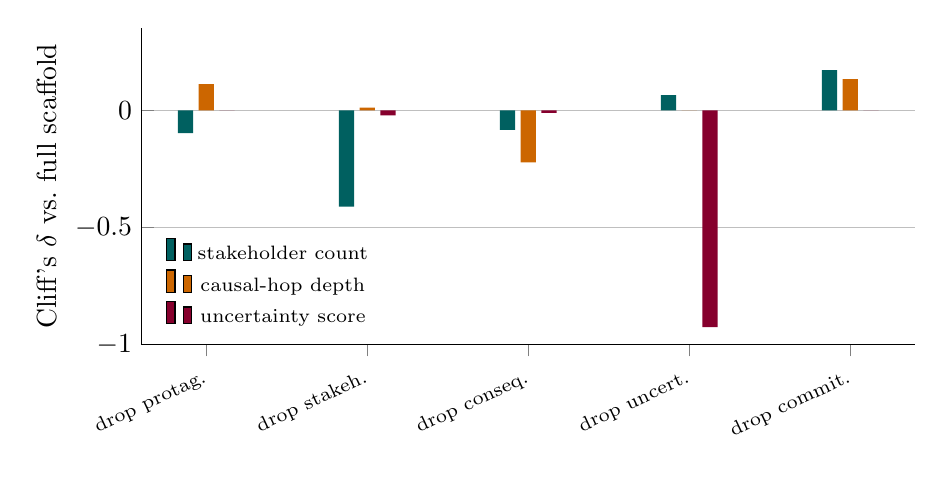
\begin{tikzpicture}
\begin{axis}[
    width=0.94\columnwidth, height=5.6cm,
    ybar,
    bar width=5.5pt,
    ymin=-1.0, ymax=0.35,
    ylabel={Cliff's $\delta$ vs.\ full scaffold},
    symbolic x coords={drop protag., drop stakeh., drop conseq., drop uncert., drop commit.},
    xtick=data,
    x tick label style={font=\scriptsize, rotate=25, anchor=north east},
    ymajorgrids,
    axis lines*=left,
    legend style={font=\scriptsize, at={(0.02,0.02)}, anchor=south west,
                  legend columns=1, draw=none, fill=none},
]
\addplot[fill=teal!75!black, draw=none] coordinates {
    (drop protag.,-0.098) (drop stakeh.,-0.411) (drop conseq.,-0.084)
    (drop uncert.,0.065) (drop commit.,0.171) };
\addplot[fill=orange!80!black, draw=none] coordinates {
    (drop protag.,0.111) (drop stakeh.,0.011) (drop conseq.,-0.222)
    (drop uncert.,0.000) (drop commit.,0.133) };
\addplot[fill=purple!70!black, draw=none] coordinates {
    (drop protag.,0.000) (drop stakeh.,-0.022) (drop conseq.,-0.011)
    (drop uncert.,-0.925) (drop commit.,0.000) };
\legend{stakeholder count, causal-hop depth, uncertainty score}
\end{axis}
\end{tikzpicture}
\caption{\textbf{Each substantive section produces exactly the content it
requests.} Section-knockout ablation (\texttt{claude-sonnet-4-6}, $n{=}90$
per cell). Cliff's $\delta$ of each drop-one-section variant against the full
scaffold, on three coded output properties. Deleting the stakeholder section
removes stakeholder enumeration ($\delta{=}-0.41$) and nothing else. Deleting
the uncertainty section removes hedging ($\delta{=}-0.93$) and nothing else.
Deleting consequence projection removes causal depth ($\delta{=}-0.22$) with
minimal spillover. Off-diagonal effects never exceed $|\delta|{=}0.17$. A
single emergent ``narrative factor'' would dilute every metric under any
knockout, and a length confound would shrink one column regardless of which
section is dropped. Neither pattern appears. (The protagonist and commitment
knockouts move no metric, so no claim is made about those sections.)}
\label{fig:attribution}
\end{figure}

% ============================== FIGURE 3 ===================================
\begin{figure}[t]
\centering
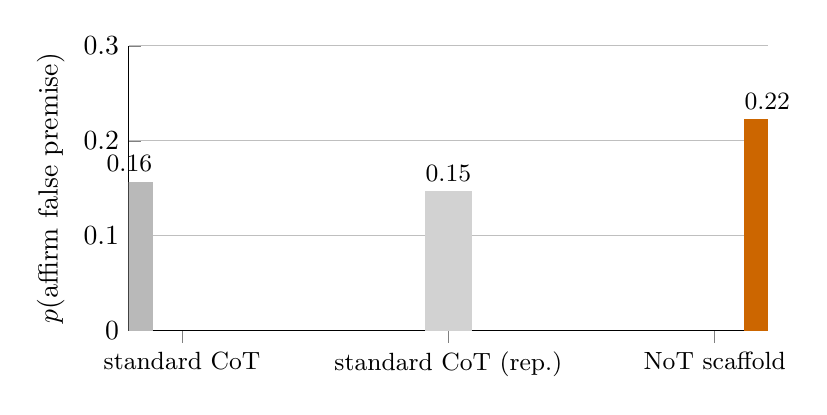
\begin{tikzpicture}
\begin{axis}[
    ybar,
    width=0.80\columnwidth, height=5.2cm,
    ymin=0, ymax=0.30,
    ylabel={$p(\mathrm{affirm\ false\ premise})$},
    symbolic x coords={standard CoT, standard CoT (rep.), NoT scaffold},
    xtick={standard CoT, standard CoT (rep.), NoT scaffold},
    x tick label style={font=\small},
    ymajorgrids,
    axis lines*=left,
    bar width=17pt,
    nodes near coords={\pgfmathprintnumber[fixed,precision=2]{\pgfplotspointmeta}},
    nodes near coords style={font=\small},
]
\addplot[fill=gray!55, draw=none] coordinates {(standard CoT,\pTrueStd)};
\addplot[fill=gray!35, draw=none] coordinates {(standard CoT (rep.),\pTrueStdRep)};
\addplot[fill=orange!80!black, draw=none] coordinates {(NoT scaffold,\pTrueNoT)};
\end{axis}
\end{tikzpicture}
\caption{\textbf{Under forced commitment the scaffold makes the
propositional failure worse, not better.} Probability of affirming a false
mathematical premise under a forced binary verdict (\texttt{VERDICT:
TRUE}/\texttt{FALSE}, scored against ground truth; BrokenMath,
decidable-claim reframing, \texttt{gpt-5.4-nano}, 100 items, 600 scored
units per arm on shared items, no stance pressure). The scaffold's bar is
the tallest. The increase over standard CoT is $+6.7$ points with a 95\%
item-clustered bootstrap CI of $[+3.3, +10.5]$, and the scaffold abstains
less than either untreated arm (26.5\% vs.\ 32.8\% and 35.2\%), so the rise
is not an artifact of differential refusal. The middle bar was generated as
an intended one-line baseline that a configuration fallback served the
standard prompt instead. It is reported as what it is, an independent
untreated replicate, and the two gray bars differ by $1.0$ point (CI
$[-1.5, +3.3]$), which bounds replicate noise. The forced format removes
every expressive channel, including hedging, shared blame, and softened
phrasing, through which a register-level intervention could simulate
improvement or harm. Movement on this measure is movement in the model's
commitments, and here it moves against the scaffold, replicating an
independent judge-scored finding on the same corpus.}
\label{fig:propositional}
\end{figure}

\end{document}
